\section{顶盖驱动方腔流}

\begin{frame}
    \begin{figure}[H]
        \centering
        \begin{tikzpicture}
            % lid driven cavity
            % draw a box
            \def\boxlength{5}
            \draw[-] (0,0)--(0,\boxlength)--(\boxlength,\boxlength)--(\boxlength,0)--cycle;
            \node at (0.5*\boxlength, -0.5) {$L$};
            \node at (-0.5, 0.5*\boxlength) {$L$};

            % u velocity
            \node at (0.5*\boxlength, 1.05*\boxlength) {$\vec{u}=1\vec{i}\rightarrow$};
            % left 3 side u = 0
            \node at (0.5, 0.5*\boxlength) {$\vec{u}=\vec{0}$};
            \node at (\boxlength-0.5, 0.5*\boxlength) {$\vec{u}=\vec{0}$};
            \node at (0.5*\boxlength, 0.5) {$\vec{u}=\vec{0}$};

            % a vortex in center of the box
            \draw[->] (0.2*\boxlength, 0.9*\boxlength) -- (0.8*\boxlength, 0.9*\boxlength);
            % draw a curve backward
            \draw[->] (0.8*\boxlength, 0.9*\boxlength) .. controls (0.7*\boxlength, 0.6*\boxlength) and (0.4*\boxlength, 0.8*\boxlength) .. (0.2*\boxlength, 0.9*\boxlength);
        \end{tikzpicture}
    \end{figure}
\end{frame}

\begin{frame}
    对于该问题的边界处理,
    我直接在壁面上布置了定速且不变位置的边界粒子,
    因为该问题流体环境致密,
    所以壁面粒子对于水体粒子有:
    强制力,压力和粘性力。
    $Re=100$:
    \begin{figure}[H]
        \centering
        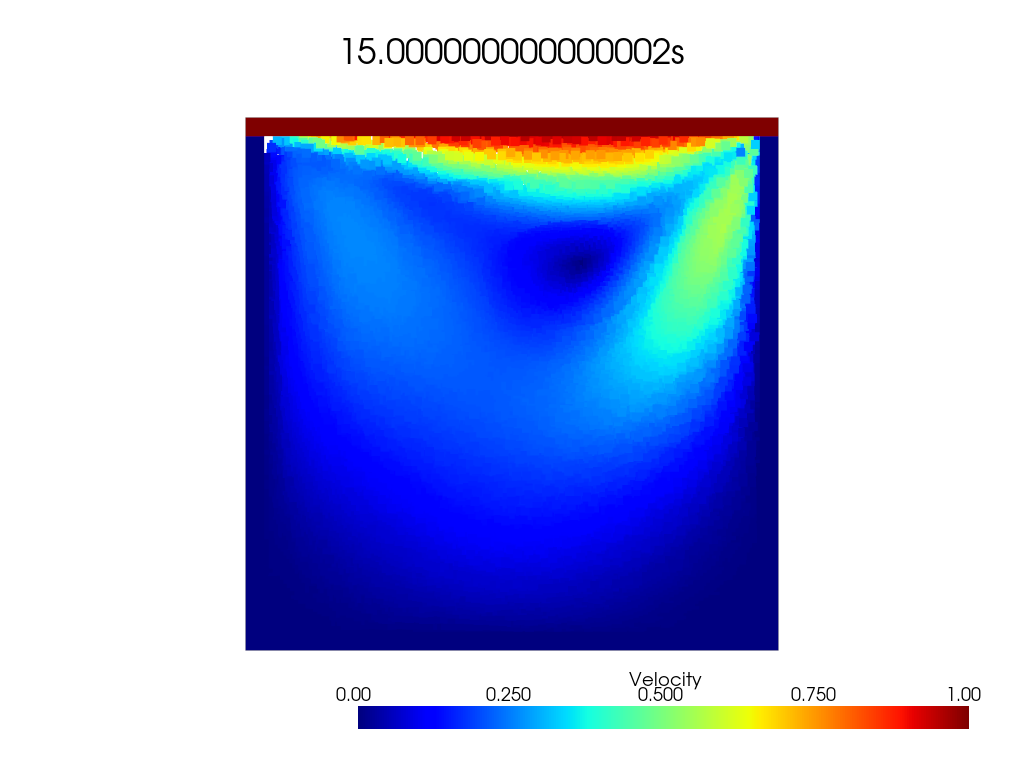
\includegraphics[width=0.8\textwidth]{images/LidDrivenCavity/Re100/lid_driven_cavity_re100.png}
    \end{figure}
\end{frame}

\begin{frame}
    \begin{figure}[H]
        \centering
        \subfigure[$N=50$]{
            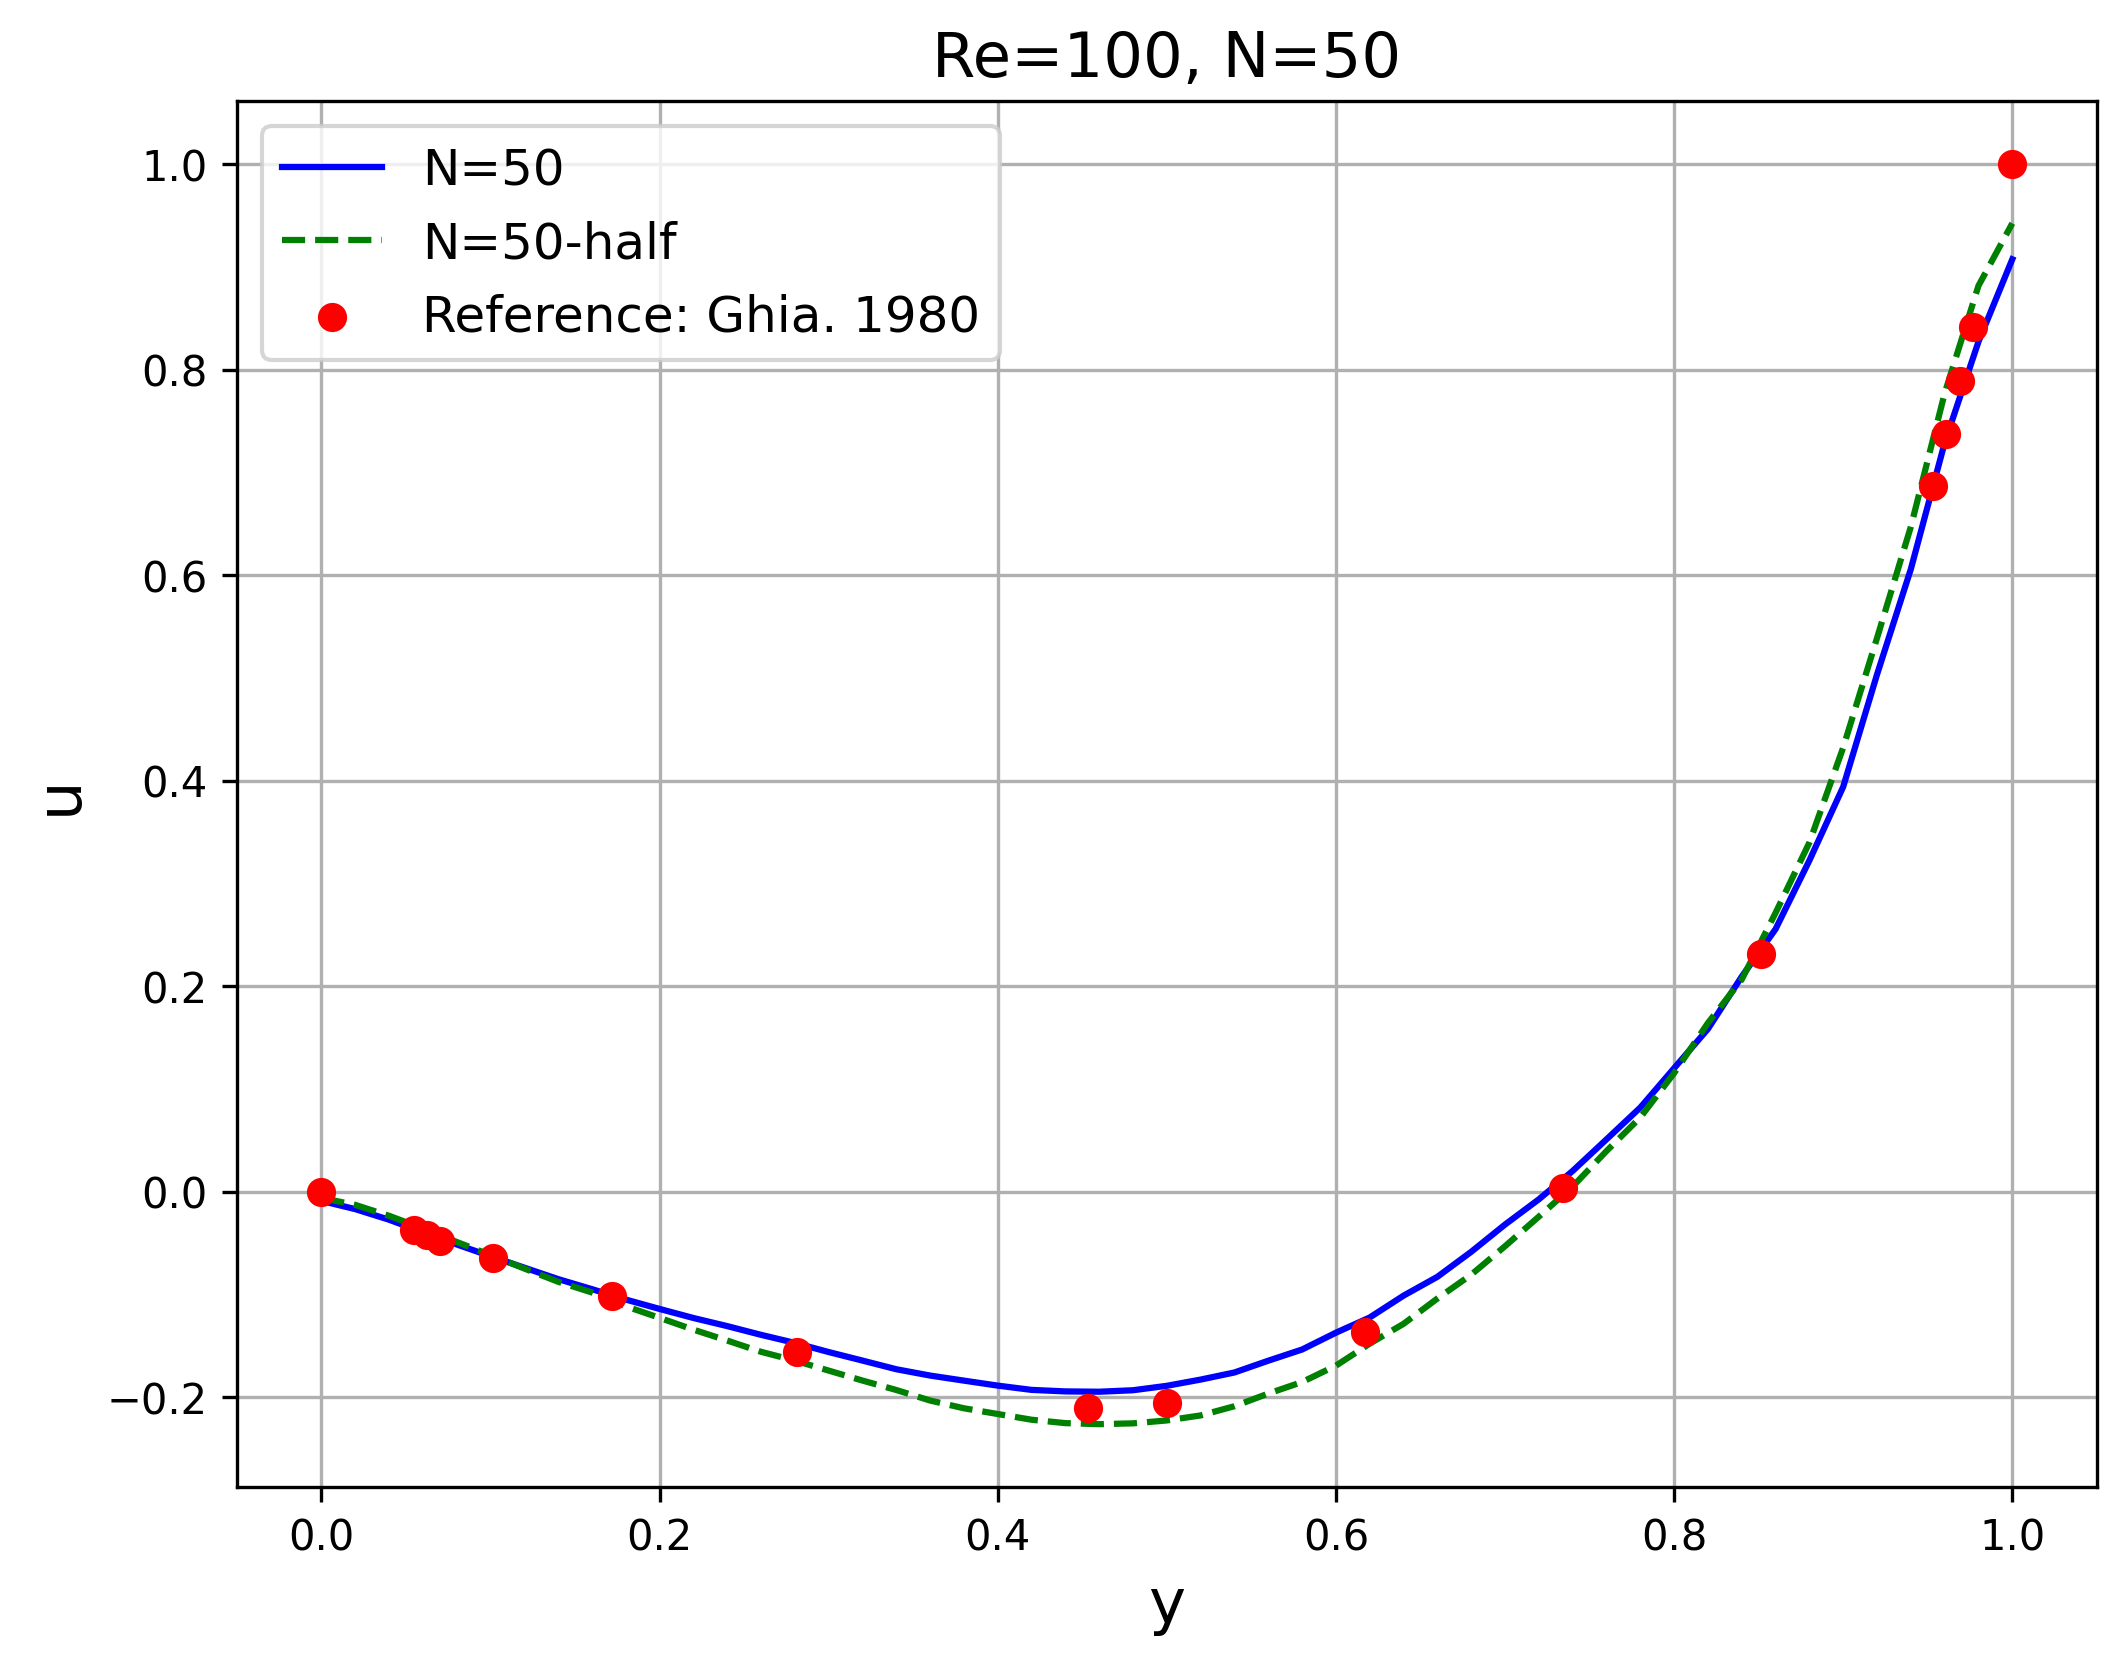
\includegraphics[width=0.45\textwidth]{images/LidDrivenCavity/Re100/u_middle_re100_N50.png}
        }
        \subfigure[$N=100$]{
            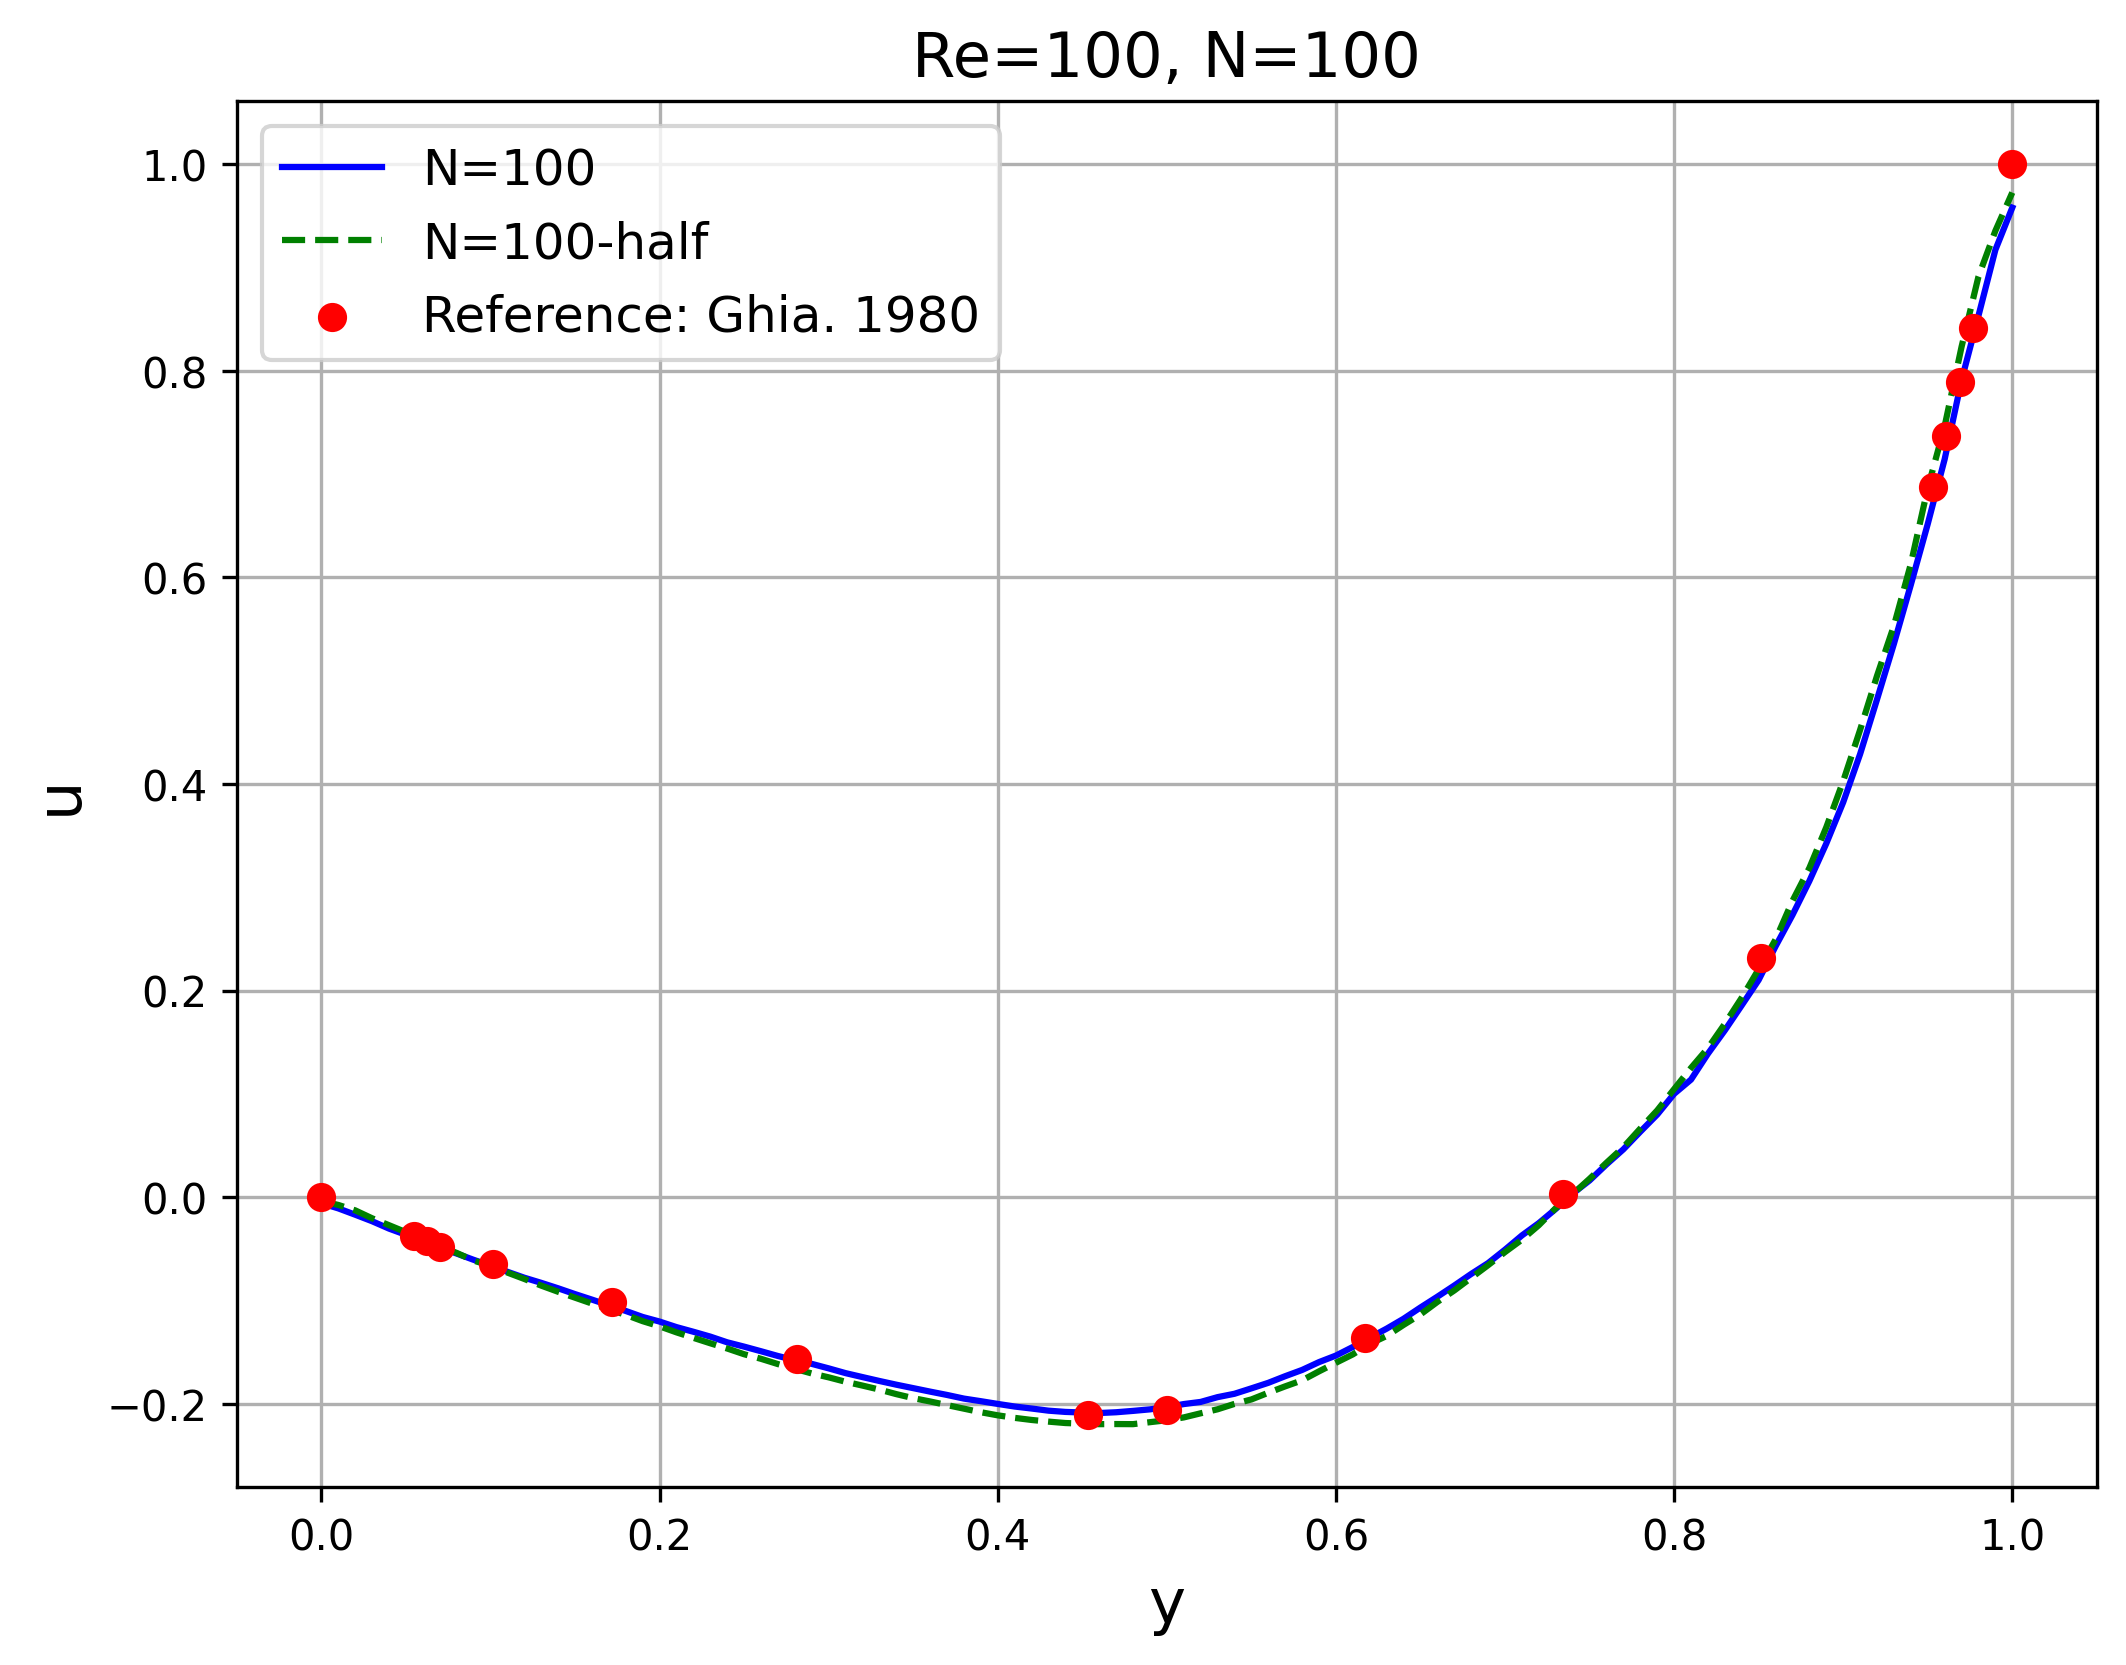
\includegraphics[width=0.45\textwidth]{images/LidDrivenCavity/Re100/u_middle_re100_N100.png}
        }
    \end{figure}
\end{frame}

\begin{frame}
    \begin{figure}[H]
        \centering
        \subfigure[$N=50$]{
            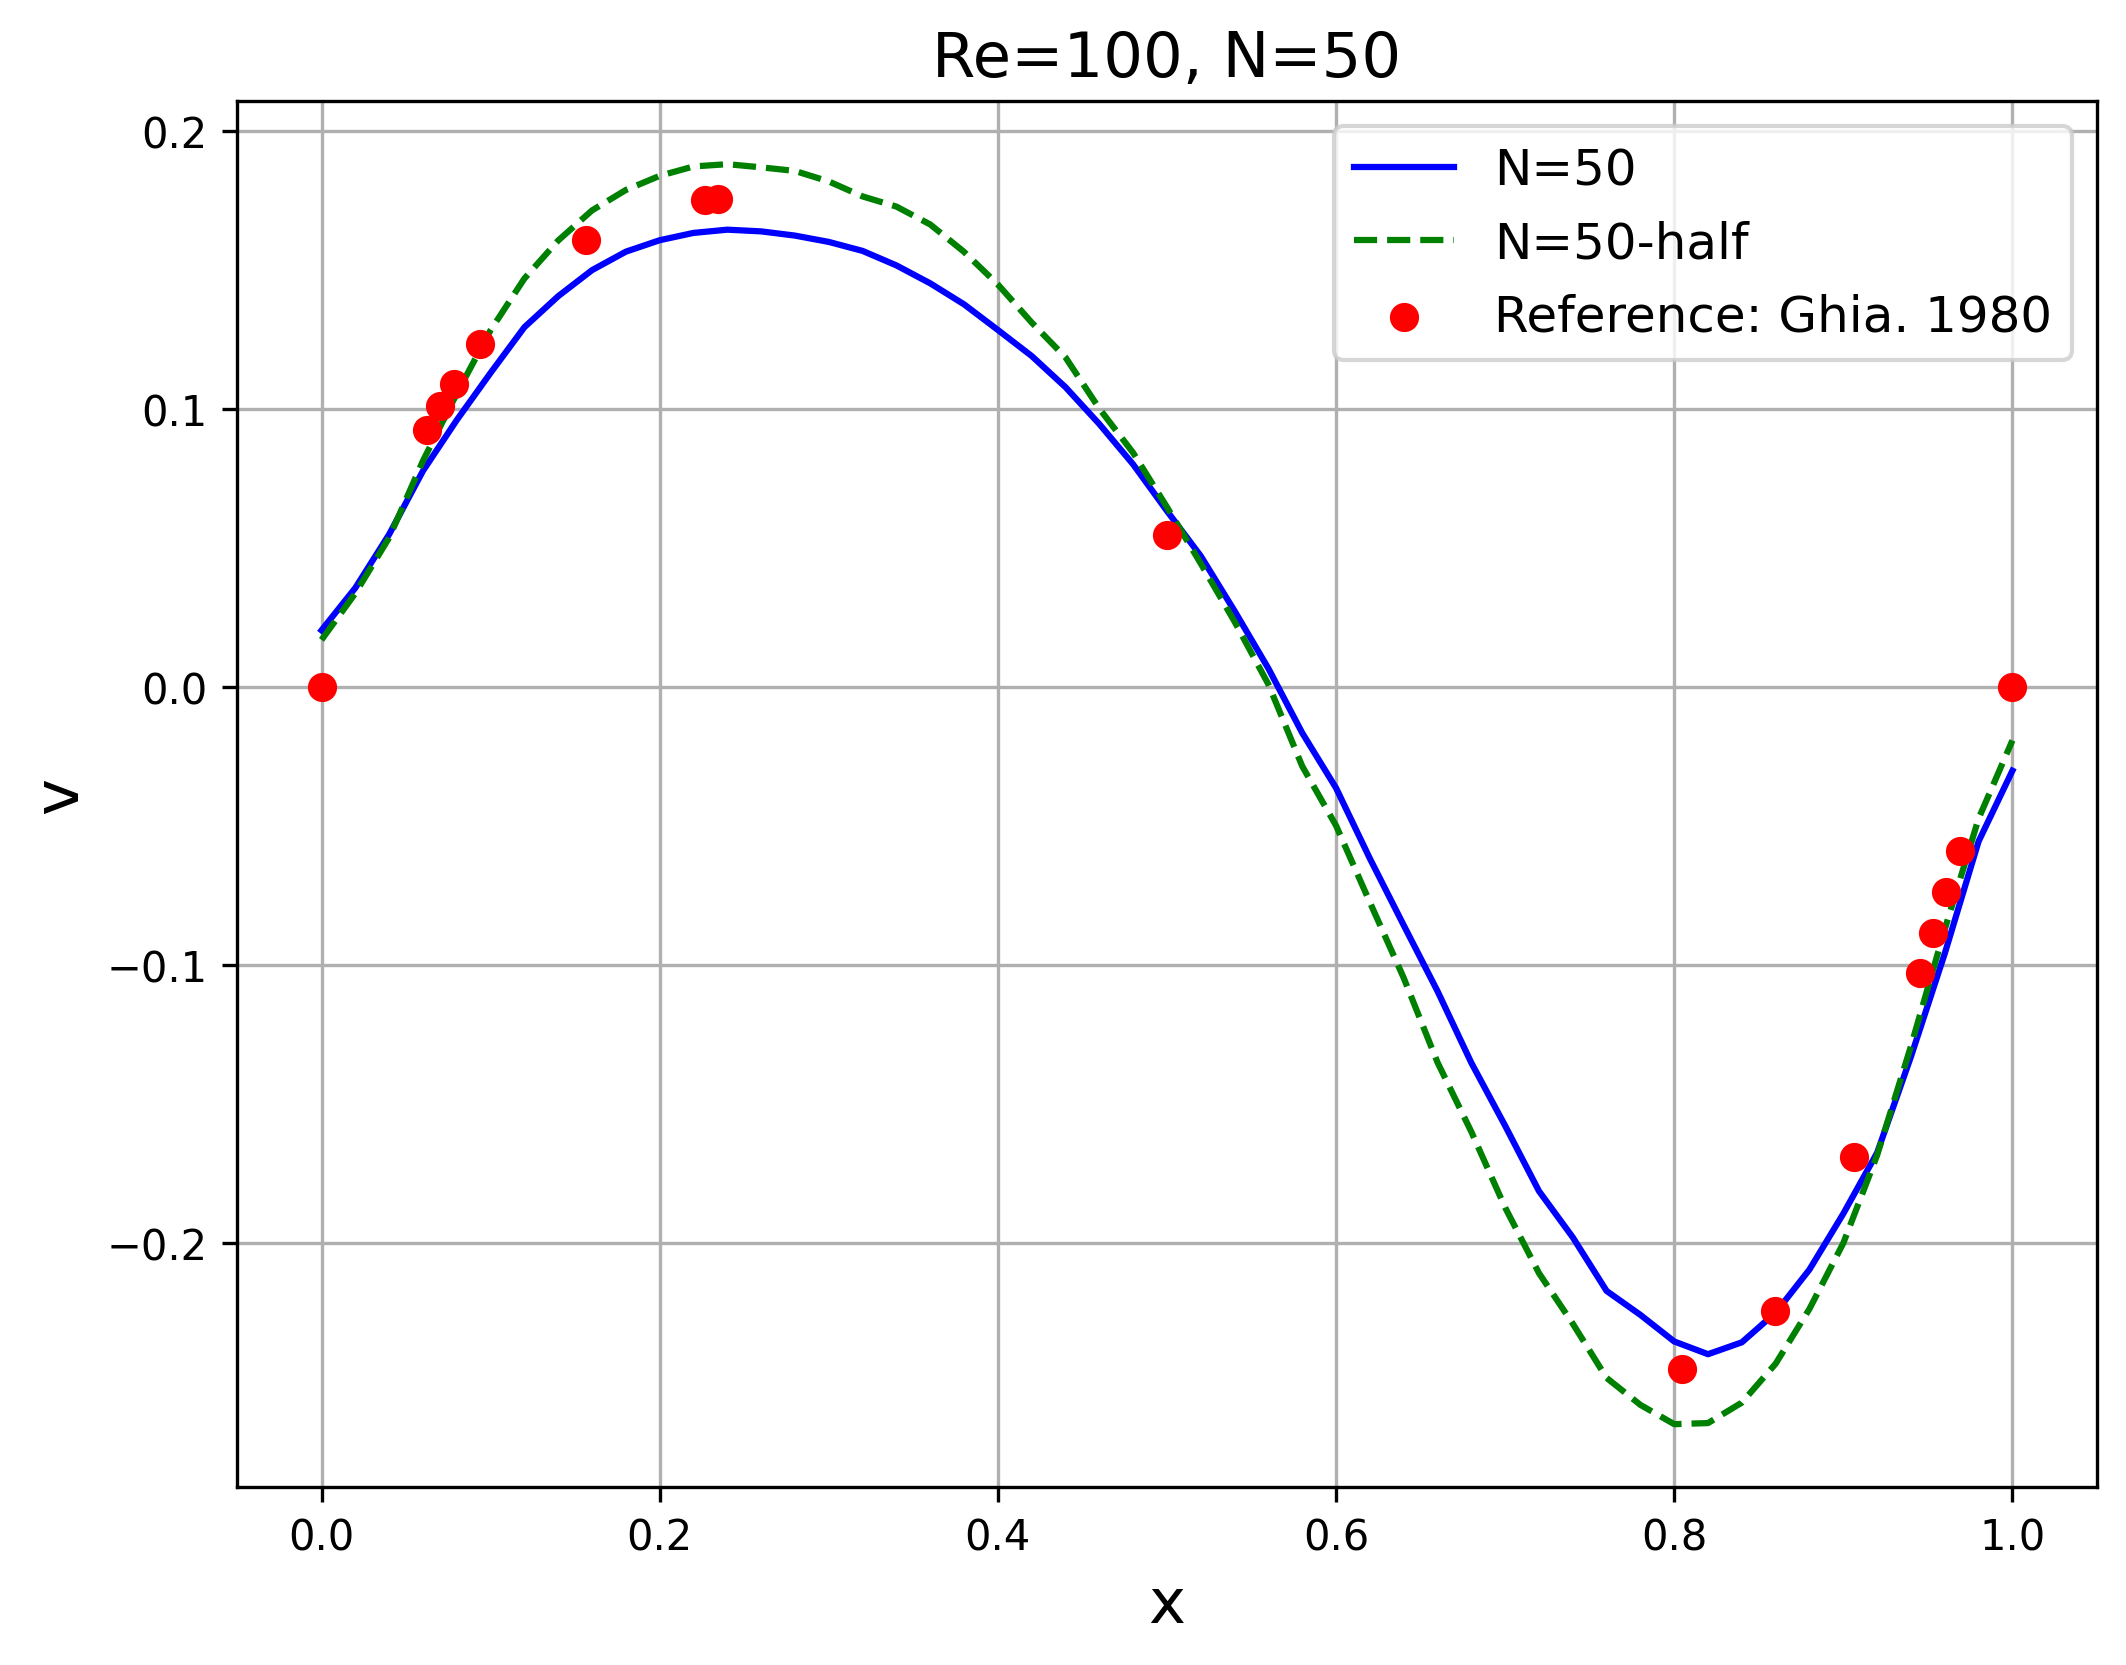
\includegraphics[width=0.45\textwidth]{images/LidDrivenCavity/Re100/v_middle_re100_N50.png}
        }
        \subfigure[$N=100$]{
            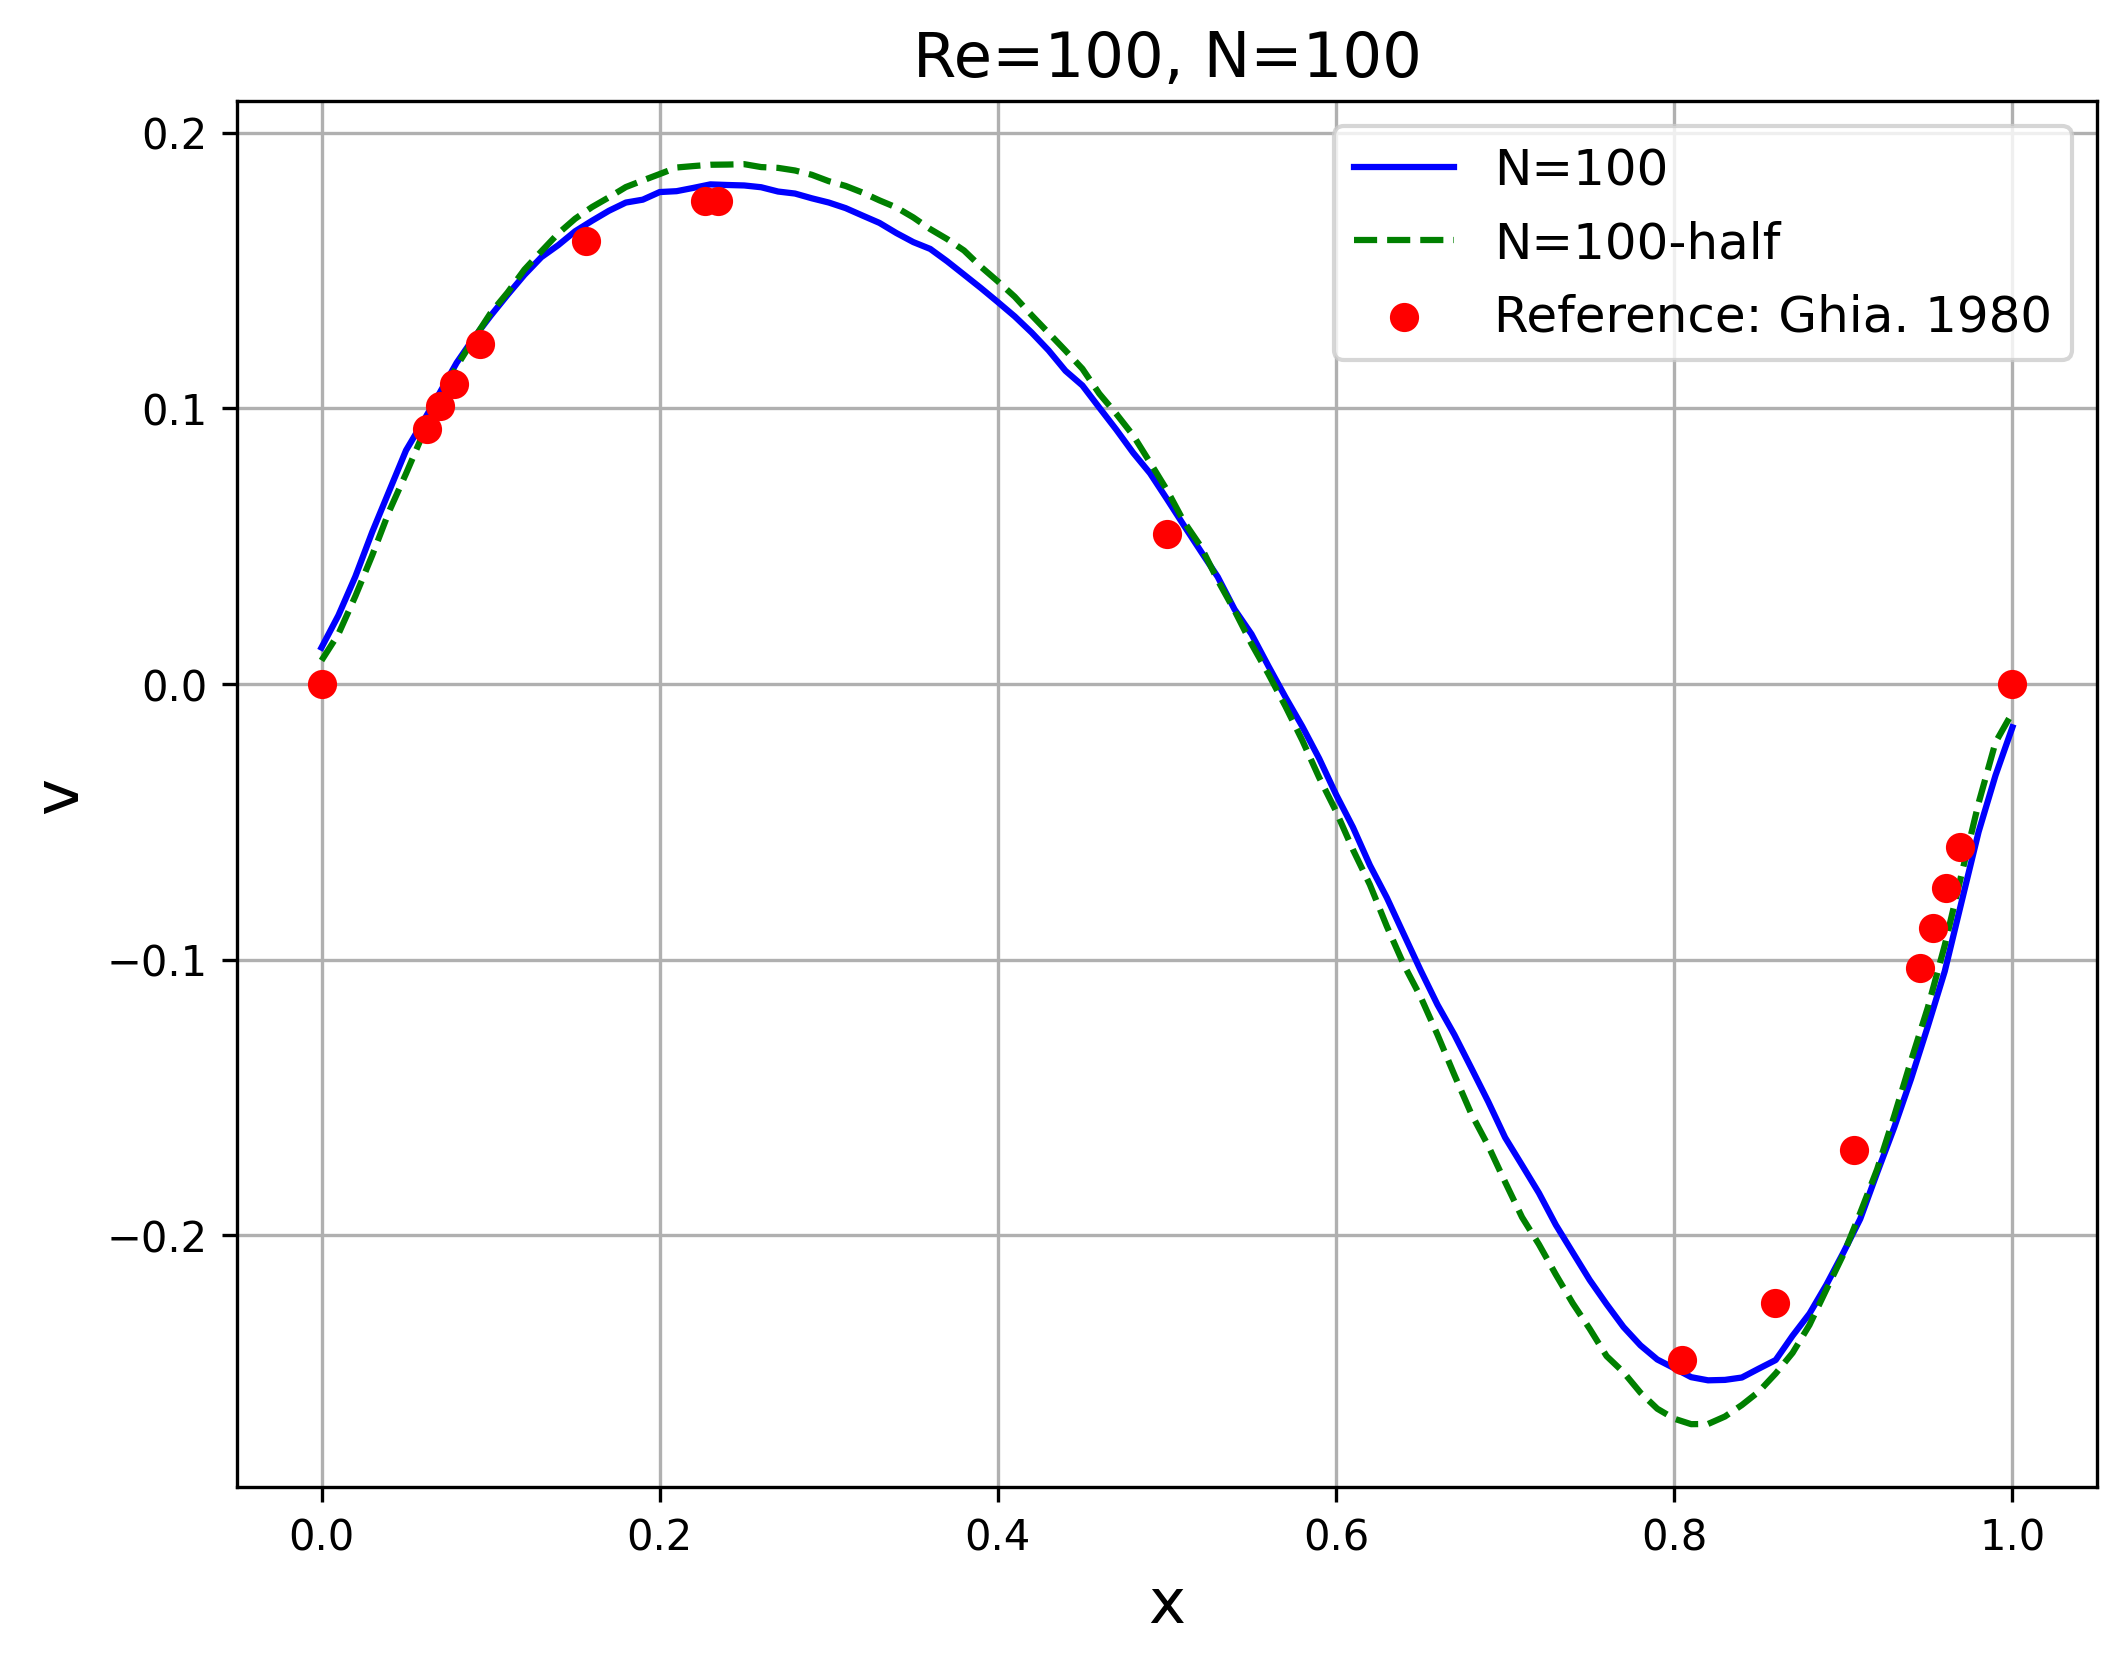
\includegraphics[width=0.45\textwidth]{images/LidDrivenCavity/Re100/v_middle_re100_N100.png}
        }
    \end{figure}
\end{frame}

\begin{frame}
    $Re=400$:
    \begin{figure}[H]
        \centering
        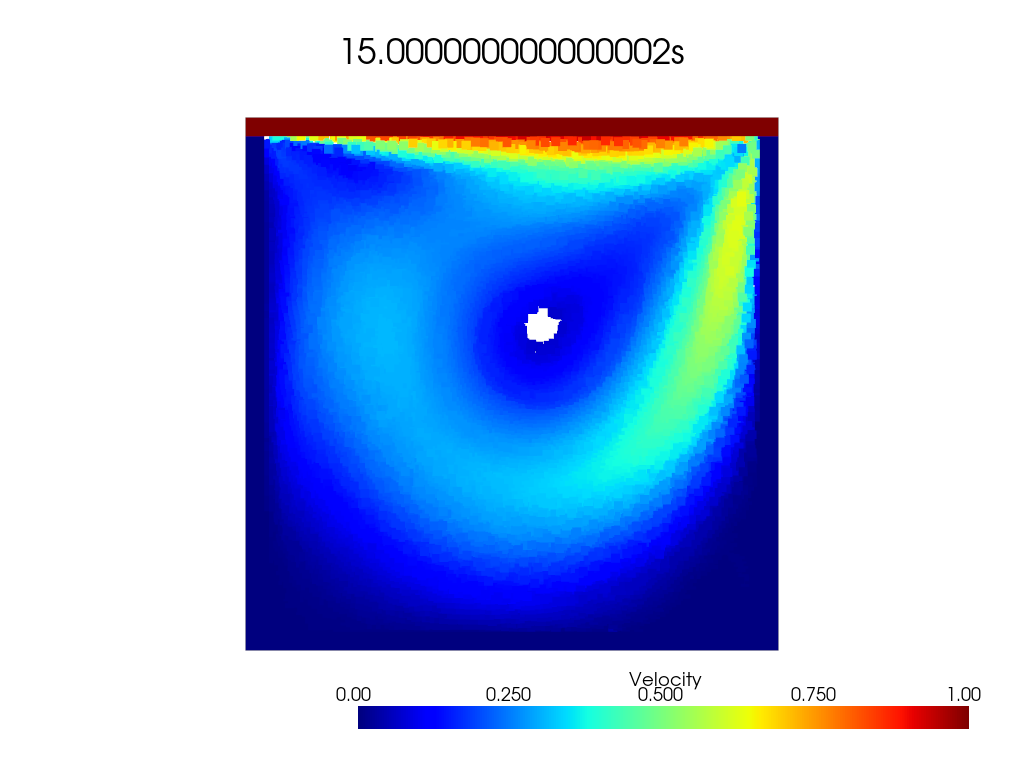
\includegraphics[width=0.8\textwidth]{images/LidDrivenCavity/Re400/lid_driven_cavity_re400.png}
    \end{figure}
\end{frame}

\begin{frame}
    \begin{figure}[H]
        \centering
        \subfigure[$N=50$]{
            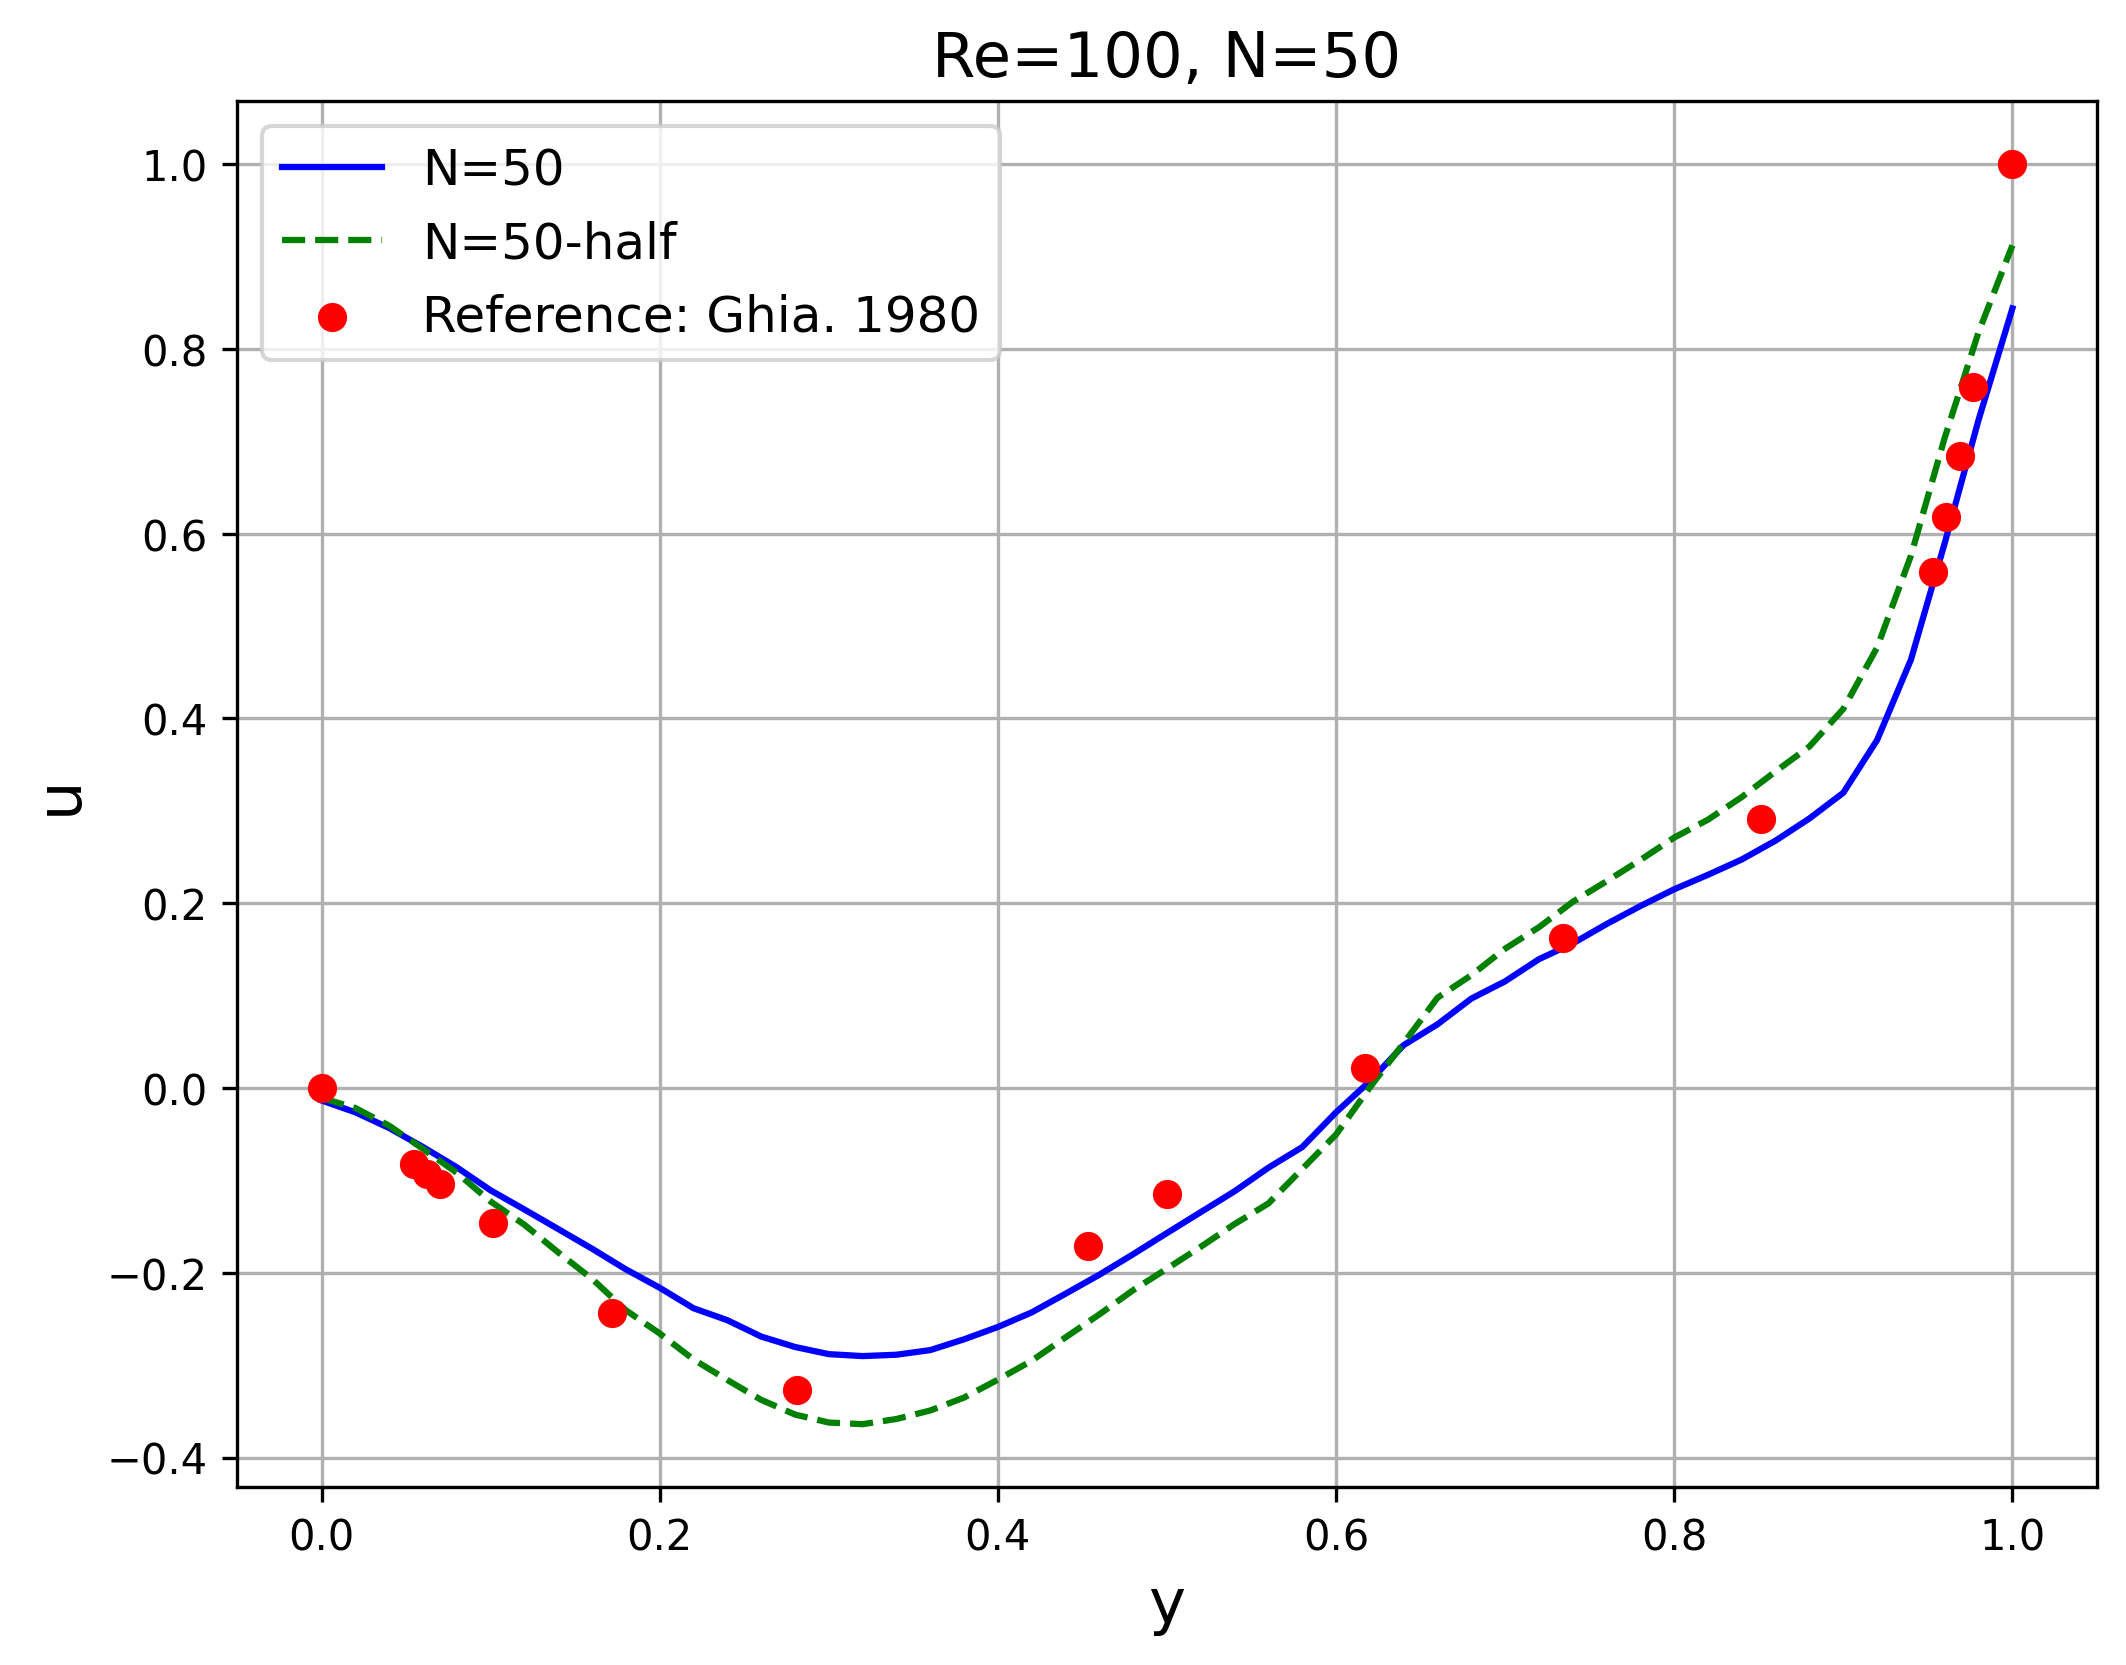
\includegraphics[width=0.45\textwidth]{images/LidDrivenCavity/Re400/u_middle_re400_N50.png}
        }
        \subfigure[$N=100$]{
            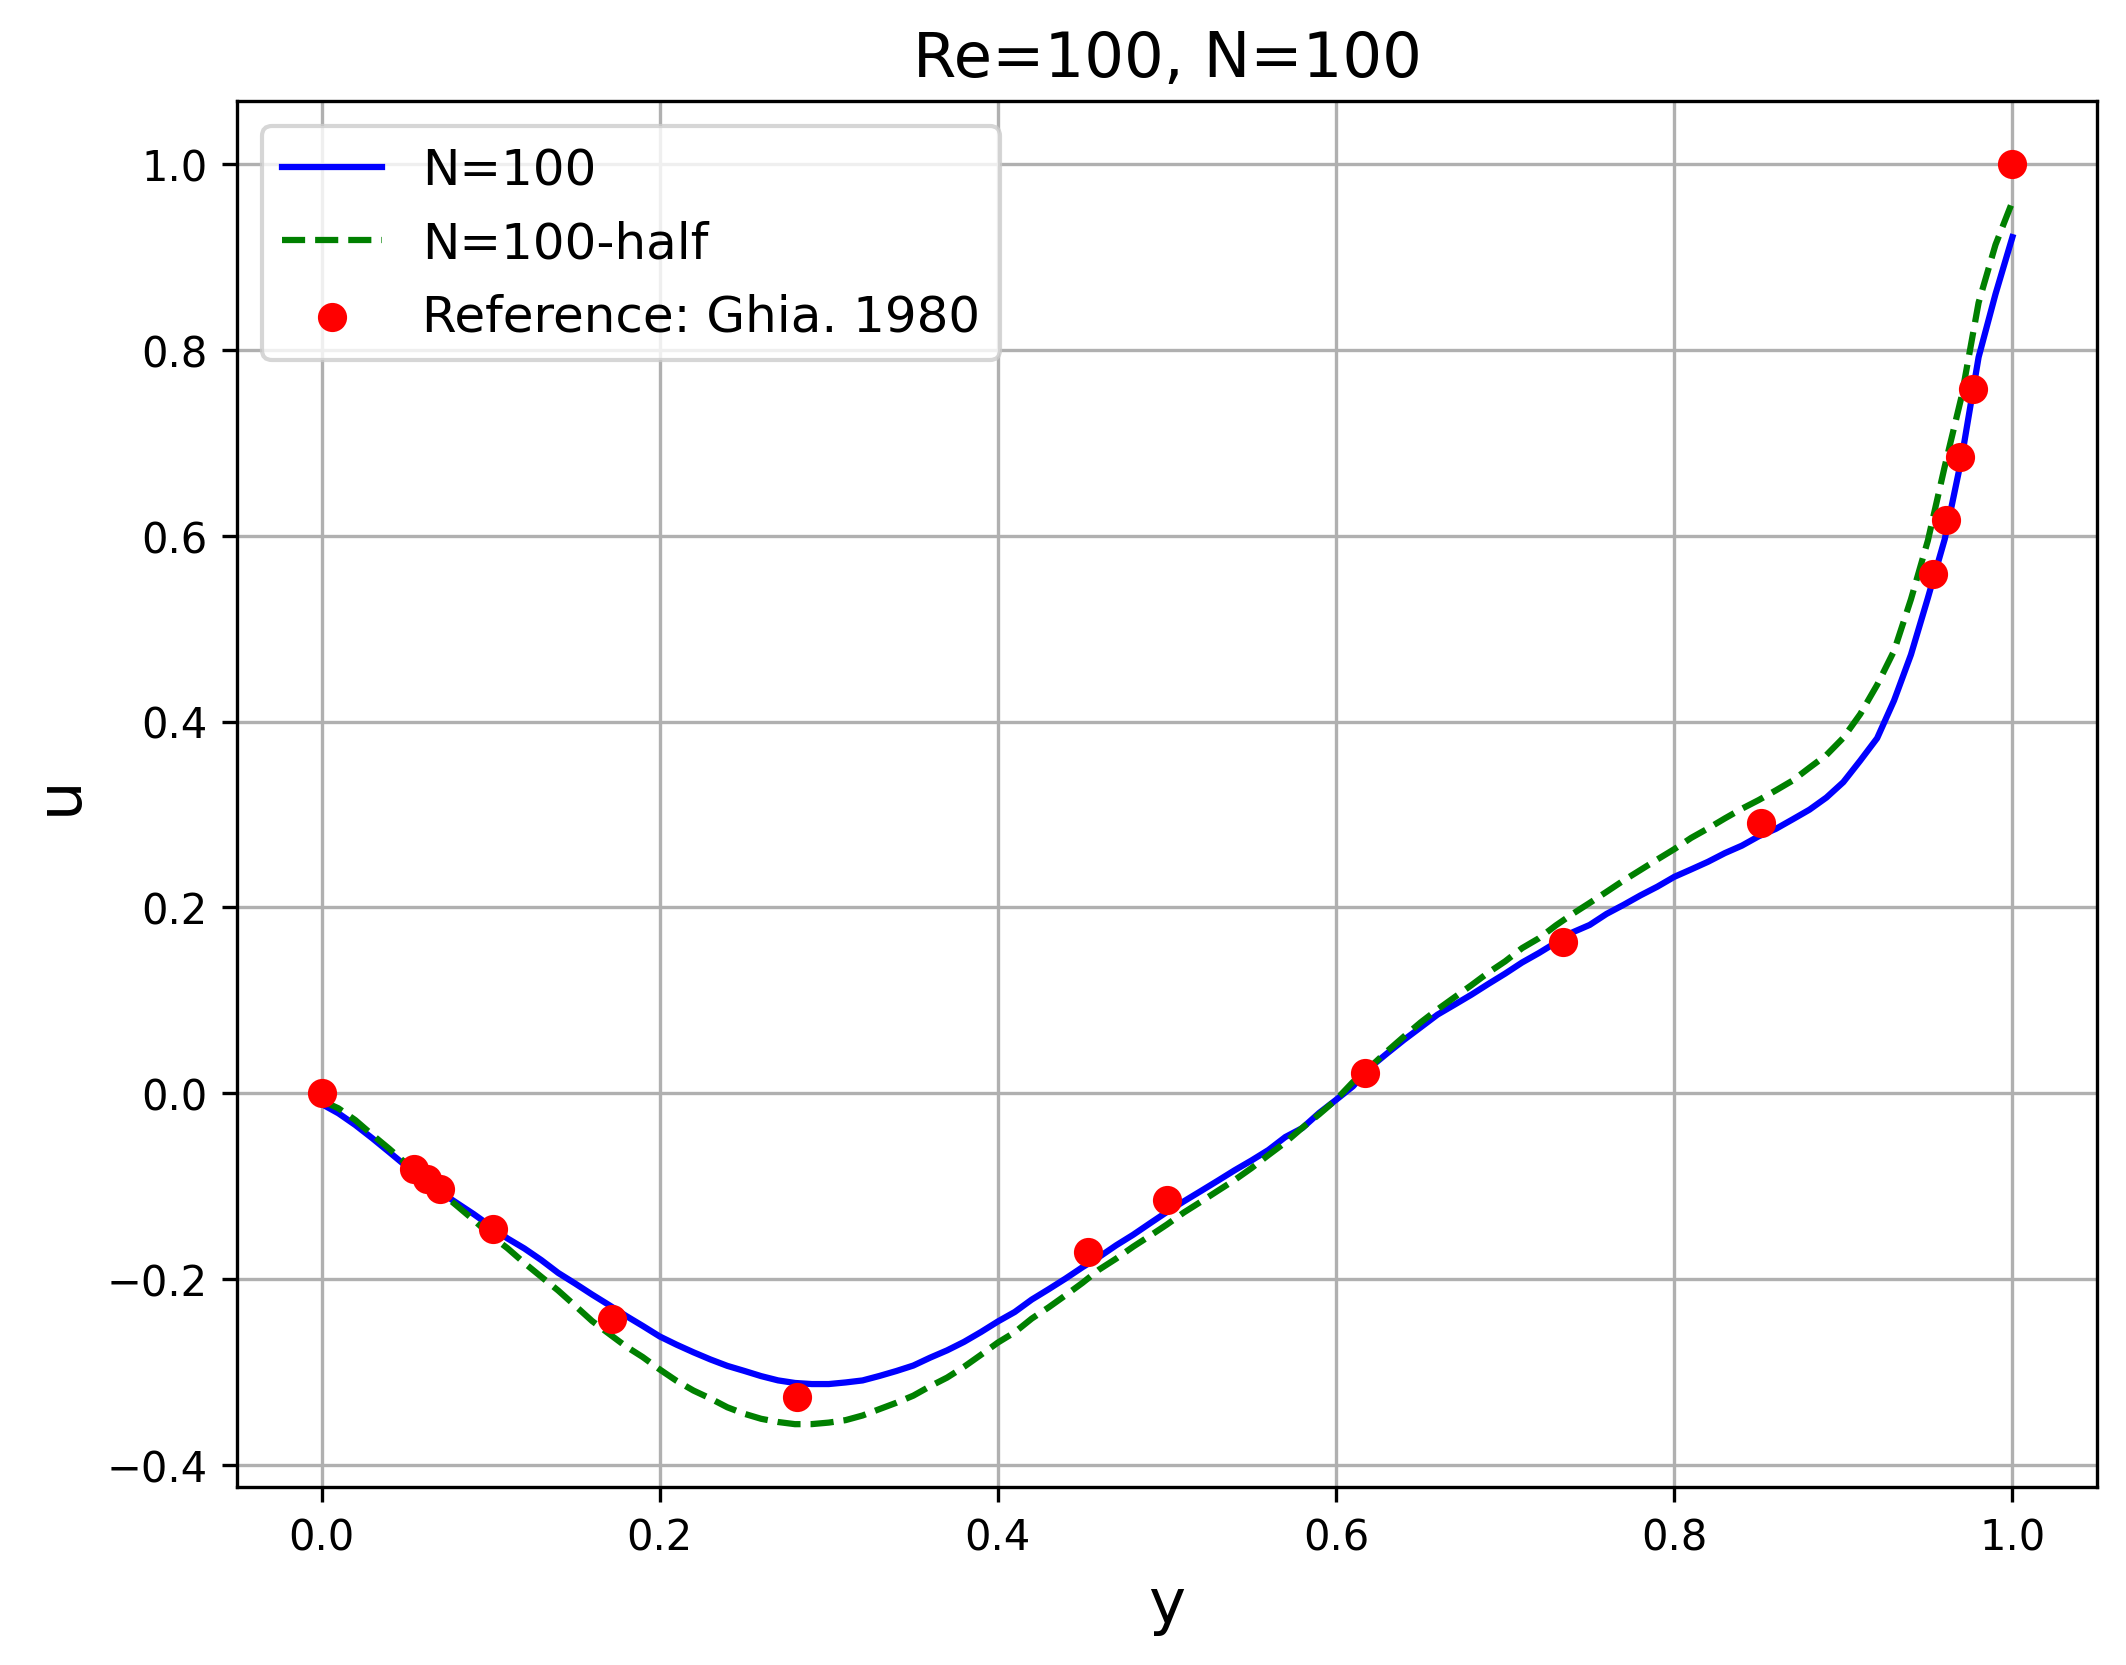
\includegraphics[width=0.45\textwidth]{images/LidDrivenCavity/Re400/u_middle_re400_N100.png}
        }
    \end{figure}
\end{frame}

\begin{frame}
    \begin{figure}[H]
        \centering
        \subfigure[$N=50$]{
            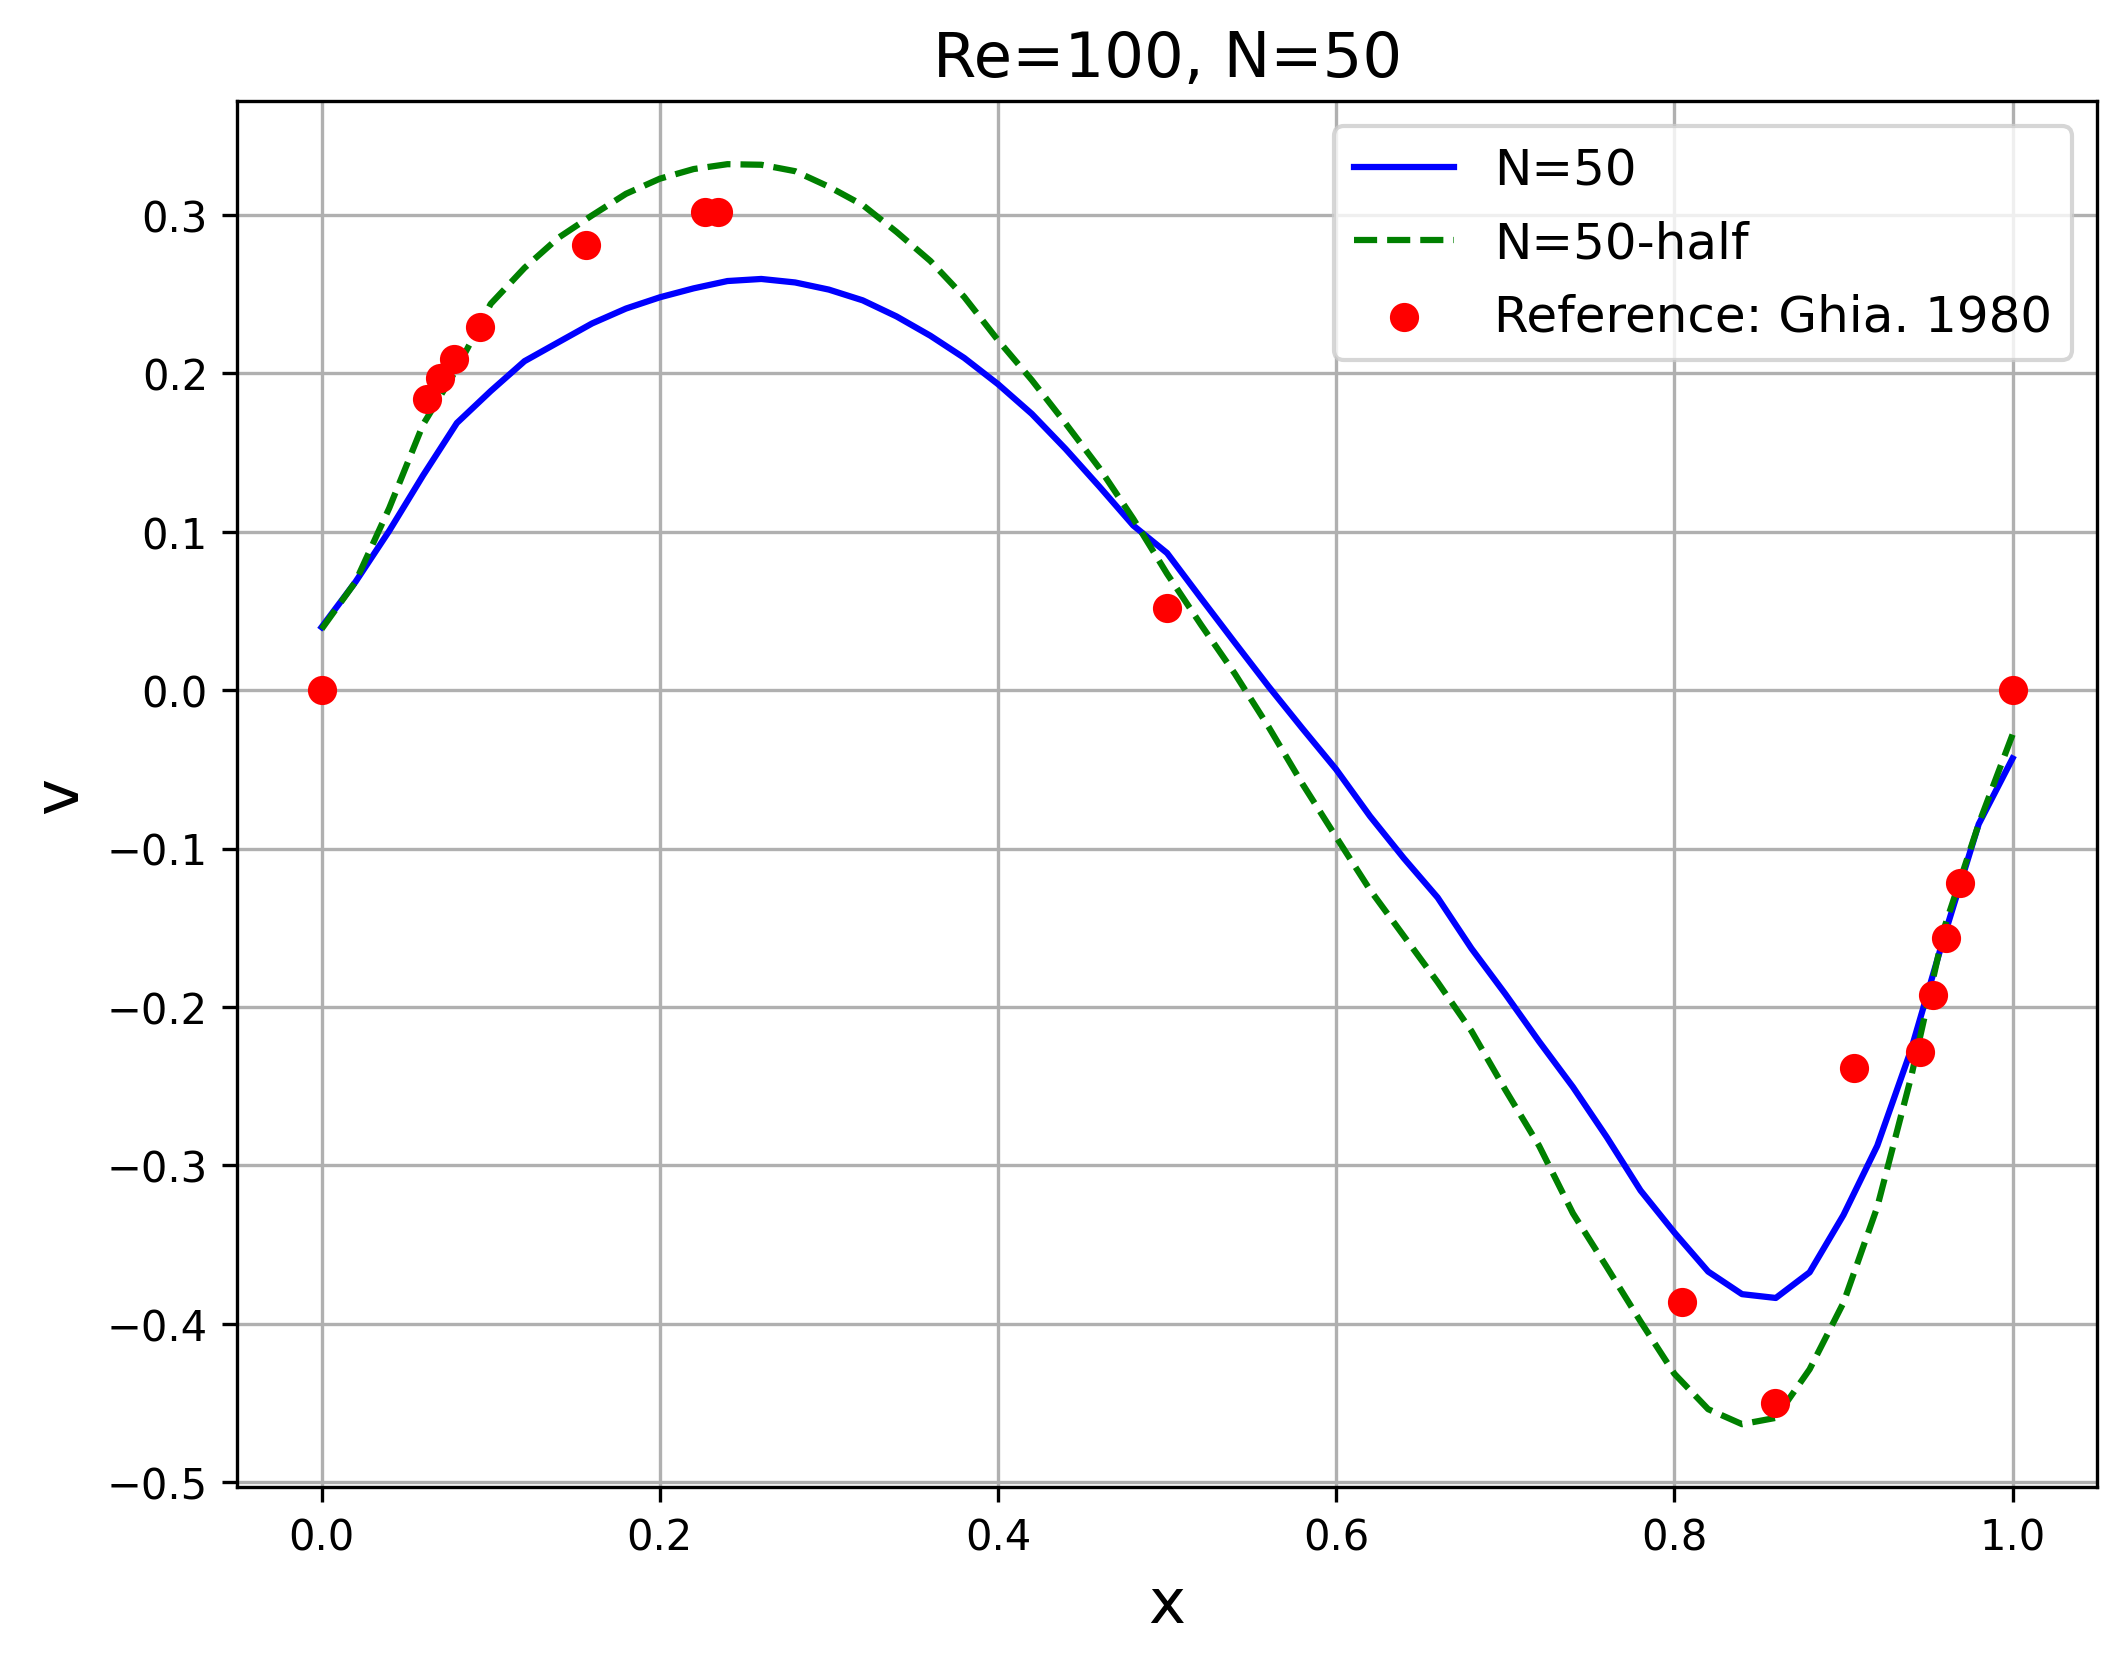
\includegraphics[width=0.45\textwidth]{images/LidDrivenCavity/Re400/v_middle_re400_N50.png}
        }
        \subfigure[$N=100$]{
            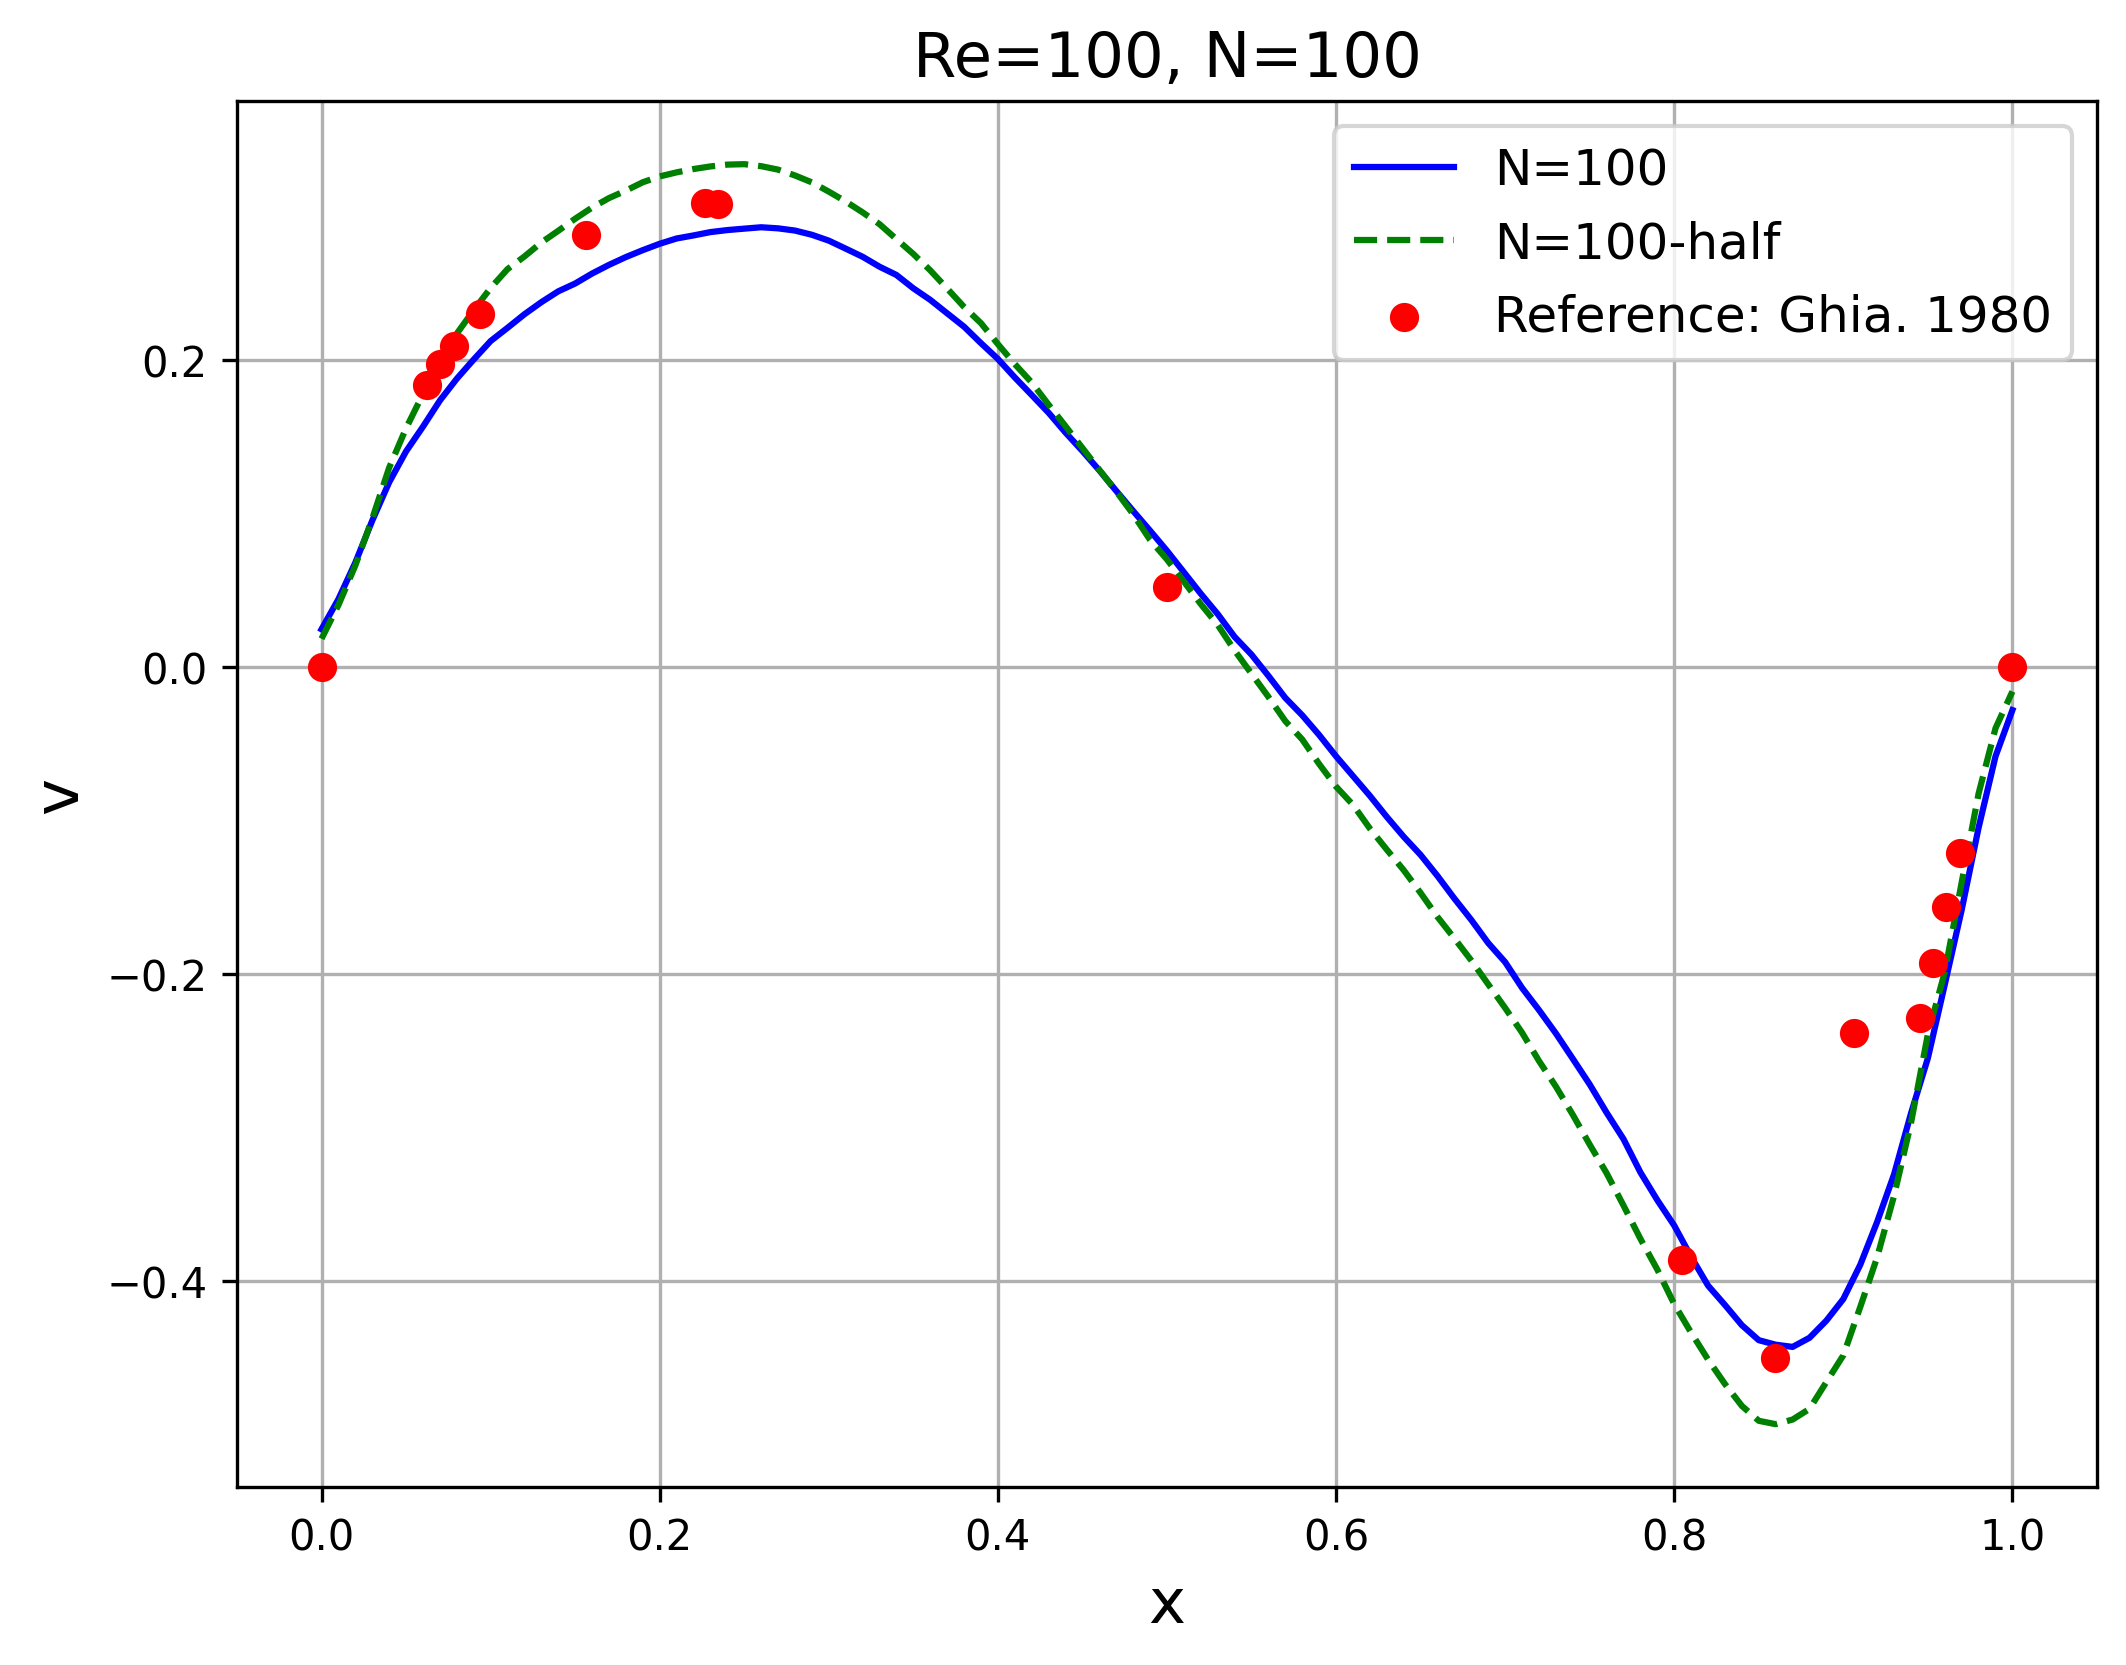
\includegraphics[width=0.45\textwidth]{images/LidDrivenCavity/Re400/v_middle_re400_N100.png}
        }
    \end{figure}
\end{frame}

\begin{frame}
    对于顶盖驱动流而言:
    \begin{itemize}
        \item 不垫高壁面粒子,会导致边界处流速仍不为零,并且增加粒子数的精度增益不明显。
        \item 垫高壁面粒子,会导致流域内部速度偏差稍大,但边界处的流速更吻合于边界设定值。
    \end{itemize}
\end{frame}